\chapter{State of the Art NER with Transformer Models}
\label{cha:ner_approaches}

Since their beginnings in the 1970s, \gls{ner} approaches have evolved mostly in parallel to general advancements in \gls{nlp}: Starting with early rule-based and knowledge-based systems, the field moved to machine-learning based approaches, often involving extensive feature-engineering. Deep-learning based approaches using neural networks and word embeddings then began to replace these architectures, making feature-engineering more and more obsolete, and allowing for richer forms of word representations. (cf. \cite{yadav_survey_2019}). 

Most recently, transformer models based on self-attention have achieved new state of the art performance for several \gls{nlp} tasks including \gls{ner}. The transformers architecture was first introduced in 2017 by \citeauthor{vaswani_2017}, in the seminal paper `Attention Is All You Need' (\cite{vaswani_2017}).

Like prior appraoches, transformers can be used to map input sequences to output sequences of the same length (cf. \cite[3]{tunstall_natural_2022}). However, they represent a clear shift from prior model architectures since they do not process their inputs sequentially. This allows for a parallelization of computations. Furthermore, transformer models represent a new way to consider the context of input words. 

\section{Self-Attention}
Transformer models use a mechanism called \textbf{self-attention} which allows them to represent each word with respect to its current context (cf. \cite[25-26]{vajjala_practical_2020}). Through self-attention, these models are able to use information from (theoretically) arbitrarily large contexts, without having to pass this information sequentially, for example through recurrent connections such as in \glspl{rnn} (cf. \cite[191]{jurafsky_2021}). 

Attention in transformer models can be conceptualized as `[comparing] an item to a collection of other items in a way that reveals their relevance in the current context.' (\cite[192]{jurafsky_2021}). Self-attention then means to compare a given item to other elements within a sequence (cf. \cite[192]{jurafsky_2021}).

When processing an input item, a backward looking self-attention layer has access to the item itself and all of the inputs before it, but not to the succeeding inputs. In bidirectional architectures such as BERT, the considered context is not limited to the preceding inputs (see \cite{devlin_2018} for further explication). 
The computation for each item in a self-attention layer is carried out independently from the computations for other input items, which allows to run a high number of computations in parallel (cf. \cite[192]{jurafsky_2021}). Transformer models thus allow for parallelization which is an advantage in terms of computational speed and efficiency compared to prior sequential approaches such as \glspl{crf}, \glspl{rnn}, or \glspl{lstm}.

\section{Key, Query, and Values}
The attention mechanism of transformer models considers each input in three different roles (cf. \cite[193]{jurafsky_2021}):

\begin{itemize}
	\item As a \textbf{query}, the input represents the current focus of attention and is compared to all of its preceding inputs (given a unidirectional, left-to-right architecture). 
	\item If the input is among the preceding inputs, it is compared to the current query, i.e. the current focus of attention. In this case, it represents a \textbf{key}.
	\item Whenever the input is used for computing the current output, it is referred to as \textbf{value}.
\end{itemize}

Figure \ref{fig:self_attention} illustrates the process of calculating the value for the third element in a sequence including the key, query, and value vectors for the current item $x_3$ and the preceding items $x_1$ and $x_2$. We can see that after generating these vectors, they key-query comparisons are carried out, which are then passed to the softmax function. The resulting values are then multiplied by the value vector, and summed up to obtain the output vector $y_3$. 

\begin{figure}[H]
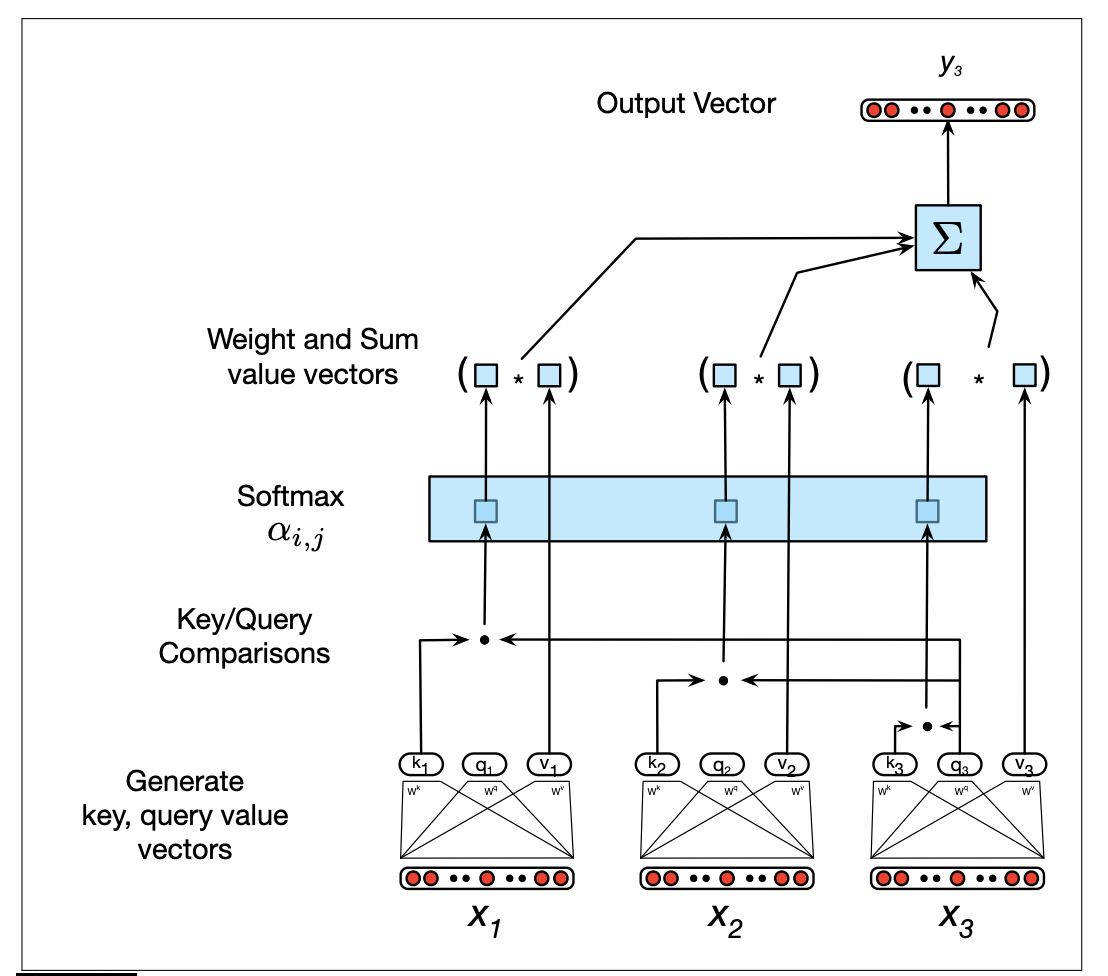
\includegraphics[width=0.8\linewidth,keepaspectratio]{images/self_attention.png}  \caption{Transformers: Key, query, value implementation in left-to-right attention, taken from \cite[194]{jurafsky_2021}}
  \label{fig:self_attention}
\end{figure}

\section{Multi-Head Attention}
By extending the concept of self-attention to multiple heads, transformer models are able to consider different aspects of relationships between input words. This mechanism is called multi-head attention, and implemented in the form of multiple, parallel self-attention layers which are located at the same depth of the network. Each of these heads learns its own parameters, allowing it to pay attention to different ways in which the words in the input relate to each other (cf. \cite[194]{jurafsky_2021}). 

\section{Transformer Blocks}
Transformer models are composed of so-called transformer blocks. All of them have the same input und output dimensions, which allows to stack them on top of each other (cf. \cite[194]{jurafsky_2021}). 

These transformer blocks are themselves multilayer networks, containing the self-attention layers, simple linear layers, and feedforward networks. As a mechanism to improve training performance, residual connections and layer normalization are implemented in each block, allowing to pass information directly to the next layer, and keeping the output values of each hidden layer in a certain range (cf. \cite[194]{jurafsky_2021}). 

\section{Limited Input Length}
The way attention is computed makes the process in transformer models expensive for long inputs: For every input, each pair of tokens needs to be compared. Against this background, most transformer models are limited to a certain input length, e.g. 512 tokens for BERT models, to keep computational cost within acceptable bounds.(cf. \cite[195]{jurafsky_2021}). 

\section{Positional Embeddings}
Furthermore, since transformer models do not work sequentially, the information about the positional context of each item in the input is lost. To provide this information, transformer models use additional positional embeddings to include this information. These embeddings are learned during training, just like the word embeddings, and encode information about the context for each input item (cf. \cite[195]{jurafsky_2021}). 

Figure \ref{fig:transf_arch} shows the original transformer architecture introduced by \cite{vaswani_2017}, with the insertion of positional embeddings (positional encodings) before the multi-head attention layers. 

\begin{figure}[H]
\centering
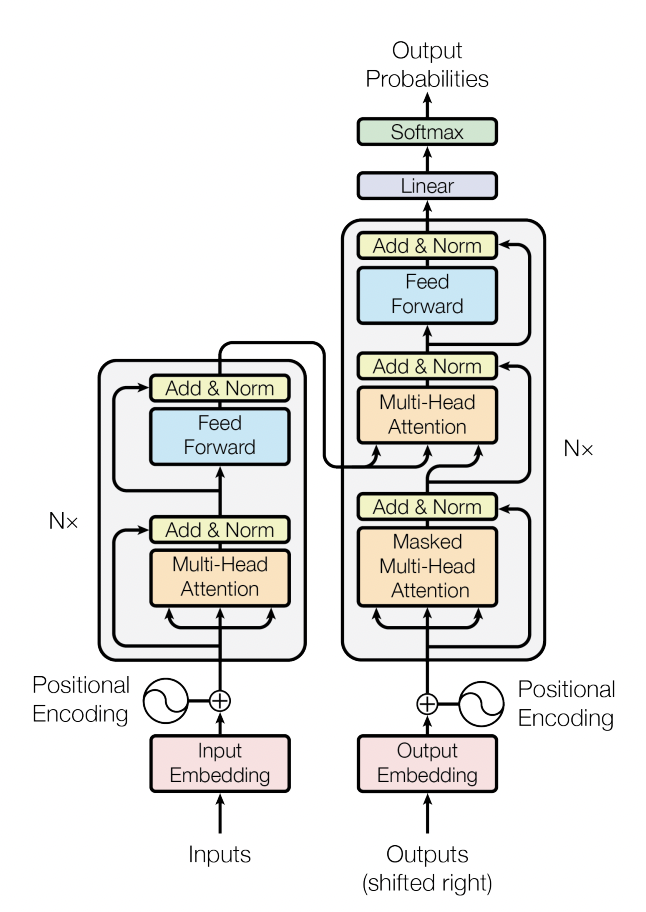
\includegraphics[width=0.6\linewidth,keepaspectratio]{images/transformer_architecture.png}  
\caption{Transformer model architecture as introduced by
\cite{vaswani_2017}}
\label{fig:transf_arch}
\end{figure}

\section{Model Architectures}
There is a large number of different architectures for transformer models, resulting in an even larger number of available models.\footnote{By the time of writing this thesis, the Hugging Face Hub lists more than 62.000 of pretrained models available for download: \url{https://huggingface.co/models}, accessed on 2022/08/06.}

The three main architectures for transformer models are encoders, decoders, and encoder-decoders. Encoder models are still the most commonly used, both in research and for business applications (cf. \cite[79]{tunstall_natural_2022}). These general architecture types can be further differentiated into different model architectures such as e.g. DistilBERT or XLM models (see \cite[79]{tunstall_natural_2022} for an overview and \cite[57-86]{tunstall_natural_2022} for details on the different architectures).

\section{Pre-Training and Fine-Tuning of Transformer Models}
Transformers are usually trained as large language models on different tasks such as \gls{nsp} or \gls{mlm}. Such pretrained language models can then be fine-tuned for downstream tasks such such as \gls{ner}.
This is achieved by first training a language model on large amounts of unlabelled text data, which is called pre-training. Pre-training allows the model to incorporate rich information about language in general, which allows it to easier learn specific tasks, called downstream tasks, on smaller datasets later. This second step is called fine-tuning. Fine-tuning requires labeled data, but can be achieved with datasets of much smaller size compared to classic supervised machine learning approaches, since the model has already achieved a lot of general knowledge about a given domain during pre-training (\cite[6-8]{tunstall_natural_2022}). 

I will explore the potentials of fine-tuning transformer models for my purpose in chapter \ref{cha:implementation} in practice. But before, I will take a closer look at existing solutions for \gls{ner}. 

%Models which have been pretrained on different corpora and can be used e.g. for fine-tuning tasks are called checkpoints. The term 'model' is thus a general term which can refer to either a a specific architectural model skeleton or a checkpoint of a pretrained model (cf. \cite{huggingface_autoclass}). 

%zusammenfassung: transformers: non-recurrent networks based on self-attention
%a self-attention layer maps input sequences to output sequences of the same length, using attention heads that model how the surrounding words are relevant for the processing of the current word
%a transformer block consists of a single attention layer followed by a feed-forward layer with residual connections and layer normalizations following each 
%transformer blocks can be stacked to make deeper and more powerful networks (28)

%\subparagraph{Transfer learning for downstream tasks with transformers}
%- large transformers used for smaller downstream tasks via transfer learning
%- transfer learning = technique where the knowledge gained while solving one problem is applied to a different but related problem
%- transformers: pre-training (training of very large transformer models, unsupervised) to predict a part of a sentence given the rest of the content so it can encode the high-level nuances of the language in it
%- models are trained on more than 40GB of textual data, scraped from the whole internet
%- this model is then fine-tuned on NLP downstream tasks, e.g. NER \cite[26]{vajjala_practical_2020}
 

%\section{Summarization}